\documentclass[10pt]{article}
\usepackage[utf8]{inputenc}
\usepackage[swedish]{babel}

\def\ordf{Edvard Carlsson}
\def\sekr{Mattias Lundström}
\def\krog{Davida Åström}
\def\fvc{Henrik Ramström}
\def\enuordf{Jakob Pettersson}
\def\sreordf{Lina Samnegård}
\def\sexm{Theo Nyman}
\def\ent{Saga Åslund}
\def\cafem{Jonathan Benitez}
\def\oph{Stephanie Bol}


\def\doctype{Handlingar} %ex. Kallelse, Handlingar, Protkoll
\def\mname{Höstterminsmötet} %ex. styrelsemöte, vårterminsmöte
\def\mnum{HT/19} %ex S02/16, E01/15, VT/13
\def\date{2019-11-12} %YYYY-MM-DD
\def\docauthor{\sekr}

\def\mtime{17:15}
\def\place{E:A}

\usepackage{../../_sektion-handlingar/e-handlingar-sek}
\usepackage{../../e-mote}
\usepackage{../../../../e-sek}

\begin{document}

\firstpage{{\doctype} till {\mname} {\mnum}}{{\date} {\mtime} i {\place}}

\tableofcontents
\newpage

\subfile{../../_sektion-handlingar/_other/guide}
\newpage

\section{Dagordning}
\subsection{Tid och plats}
\tidplats

\subsection{Föredragningslista}
\begin{paralist}
    \pli{TaFMÖ}{}
    \pli{Val av mötesordförande}{}
    \pli{Val av mötessekreterare}{}
    \pli{Godkännande av tid och sätt}{}
    \pli{Val av två justeringspersoner}{}
    \pli{Adjungeringar}{}
    \pli{Godkännande av dagordningen}{}
    \pli{Föregående sektionsmötesprotokoll}{}
    \pli{Meddelanden}{}
    \pli{Beslutsuppföljning}{}

%%%% DETTA MÅSTE GÖRAS

    \pli{Övrigt}{}
    \pli{TaFMA}{}
\end{paralist}

\begin{signatures}{2}
    \emph{I Sektionens tjänst}
    \signature{\ordf}{Ordförande}
    \signature{\sekr}{Kontaktor}
\end{signatures}

\subfile{../ekonomi/ekonomisk_rapport.tex}
\newpage
%\addcontentsline{toc}{subsection}{Balansrapport}
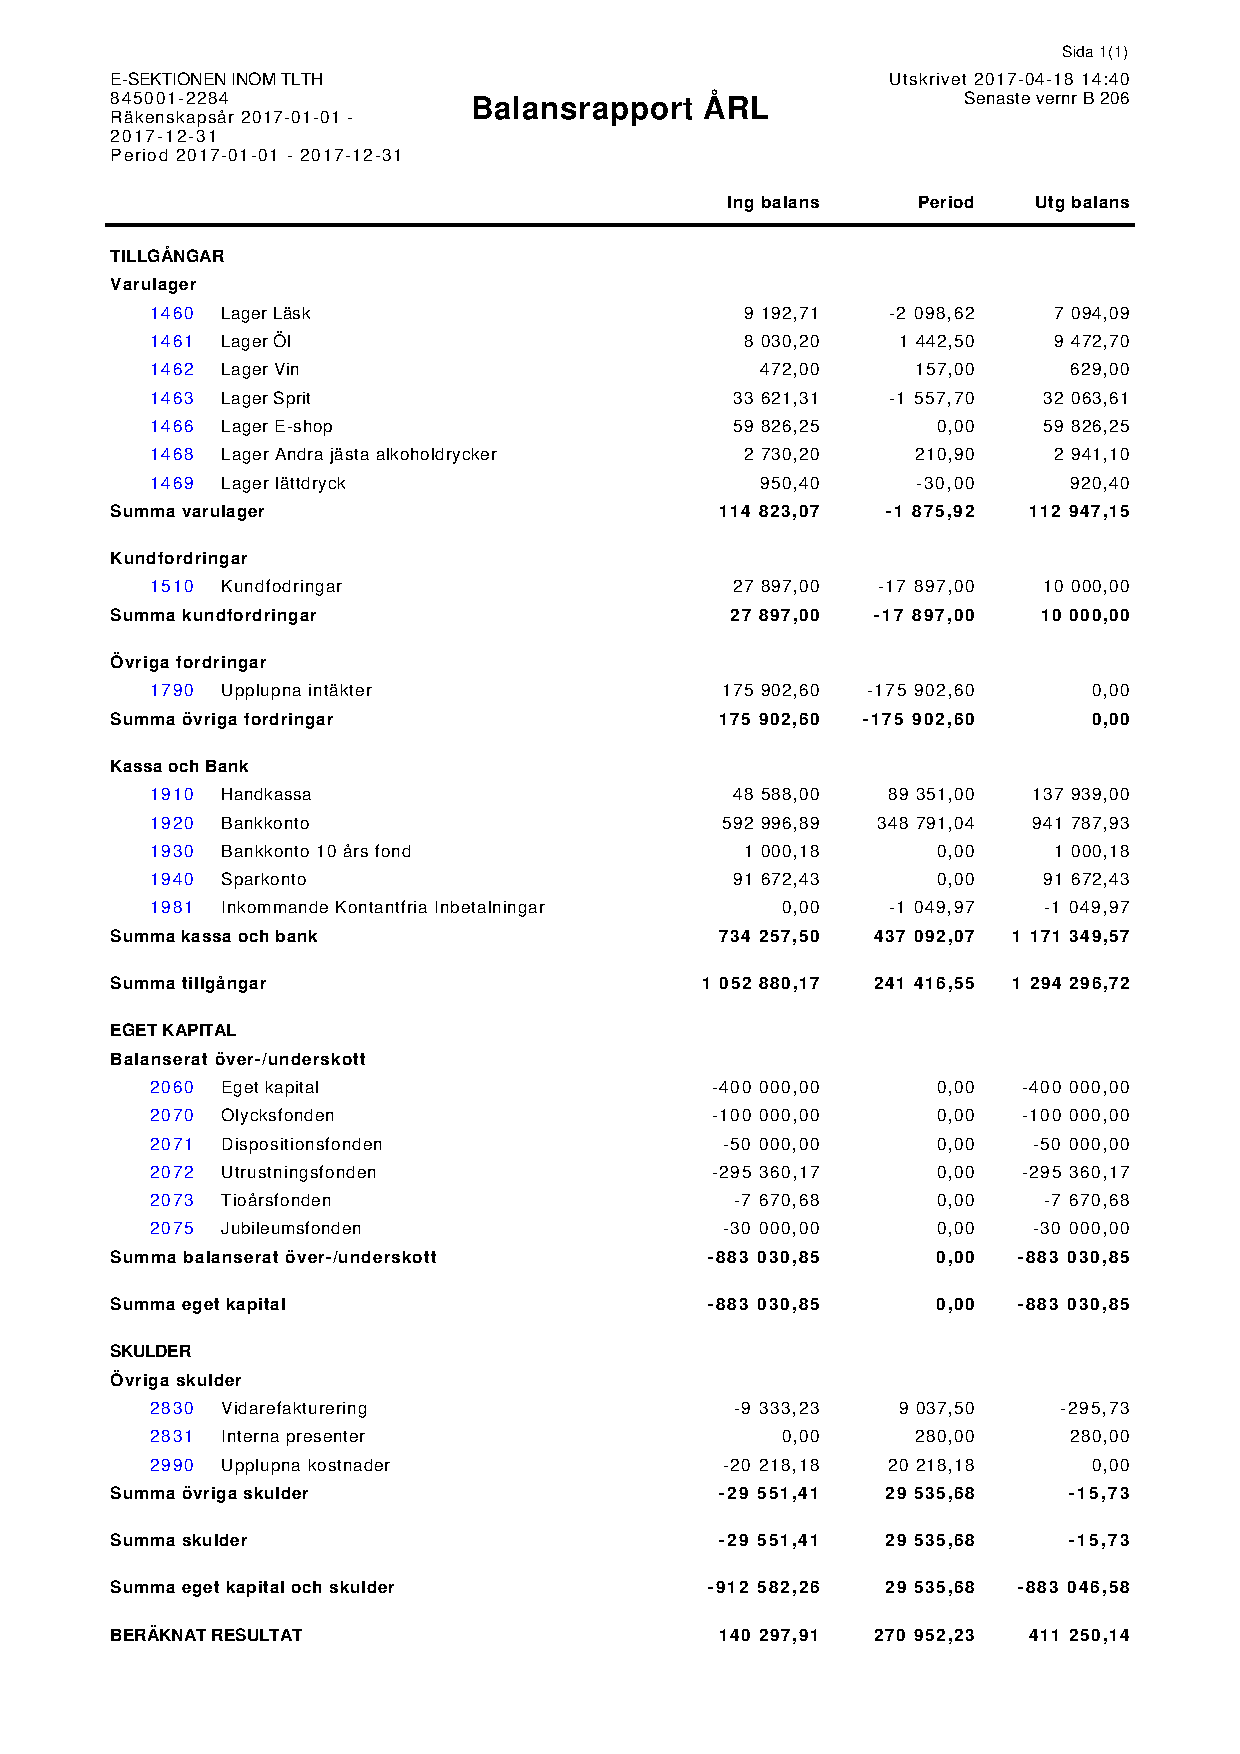
\includepdf[pages=1]{../ekonomi/balansrapport.pdf}

\subfile{../ekonomi/uttag.tex}
\newpage

\begin{supersection}{Beslutsuppföljning}{}
    \subsection{Överblick}
    \begin{busek}
    \beslutsek{VTM/19}{Renovering av Biljard}{Adam Belfrage}{\SI{35000}{kr} för en större renovering av Biljard}{HTM/19}
    \beslutsek{VTM/19}{Inköp av cykelvagn}{Davida Åström}{}{HTM/19}
    \beslutsek{VTM/19}{Inköp av utrustning för Elektro Banana Band}{William Sjödin, Daniel Bakic, Oskar Magnusson, Valter Möller}{Ska vi skriva beskrivninagar?}{HTM/19}
    \beslutsek{VTM/19}{Inköp av iZettle scanners}{Davida Åström}{}{HTM/19}
    \beslutsek{VTM/19}{Inköp av kameratillbehör}{Sonja Kenari}{}{HTM/19}
    \beslutsek{VTM/19}{Inköp av ljudteknik}{David Karlsson, Emil P. Lundh, Moa Rönnlund}{}{HTM/19}
    \beslutsek{VTM/19}{Router och Switchar för DreamHackE}{Vincent Palmer, Marcus Oknelid}{}{HTM/19}
    
   
\end{busek}


    \newpage
    \subfile{../beslutsuppf/biljard.tex}
    \subfile{../beslutsuppf/cykelvagn.tex}
    \subfile{../beslutsuppf/elektro_banana_band.tex}
    \subfile{../beslutsuppf/izettle.tex}
    \subfile{../beslutsuppf/kamera.tex}
    \subfile{../beslutsuppf/router.tex}
\end{supersection}

\begin{utskottsrapporter}
    \subfile{../utskottsrapporter/styrelsen.tex}    
    \subfile{../utskottsrapporter/cm.tex}
    \subfile{../utskottsrapporter/fvu.tex}
    \subfile{../utskottsrapporter/infu.tex}
    \subfile{../utskottsrapporter/km.tex}
    \subfile{../utskottsrapporter/nollu.tex}
    \subfile{../utskottsrapporter/enu.tex}  
    \subfile{../utskottsrapporter/noju.tex}    
    \subfile{../utskottsrapporter/sexet.tex}    
    \subfile{../utskottsrapporter/sre.tex}  
    \subfile{../utskottsrapporter/vb.tex}    
  
\end{utskottsrapporter}

\begin{supersection}{Verksamhetsplaner}{}
	\subfile{../verksplaner/2019} % Sometimes(??) gives error. Ignore?
\end{supersection}

\begin{supersection}{Uppföljningar av verksamhetsplaner}{}
	\subfile{../verksplanuppfar/2019-vt}
	\subfile{../verksplanuppfar/2019-ht}
\end{supersection}

% begin{valforslags}
%    %\subfile{../valforslag/example}
% \end{valforslags}

% \begin{berattelser}
%    %\subfile{../berattelser/example}
% \end{berattelser}

% \begin{stadgeandringar}
%    %\subfile{../stadgeandringar/example}
% \end{stadgeandringar}

\begin{motioner}
    \subfile{../motioner/booster.tex}
    %\subfile{../motionssvar/booster.tex}

    \subfile{../motioner/sasbudget.tex}
    \subfile{../motionssvar/sasbudget.tex}

    \subfile{../motioner/kroke.tex}
    \subfile{../motionssvar/kroke.tex}

    \subfile{../motioner/prefmastare.tex}
    \subfile{../motionssvar/prefmastare.tex}

    %\subfile{../motioner/toa.tex}
    %\subfile{../motionssvar/toa.tex}

    \subfile{../motioner/banan.tex}
    \subfile{../motionssvar/banan.tex}

    \subfile{../motioner/EBB.tex}
    \subfile{../motionssvar/EBB.tex}

    \subfile{../motioner/karnevalsmalaj.tex}
    \subfile{../motionssvar/karnevalsmalaj.tex}

    \subfile{../motioner/subwoof.tex}
    \subfile{../motionssvar/subwoof.tex}

    \subfile{../motioner/tandemcykel.tex}
    \subfile{../motionssvar/tandem.tex}

    %\subfile{../motioner/elbjorn.tex}
    %\subfile{../motionssvar/elbjorn.tex}

\end{motioner}

\begin{propositioner}
    \subfile{../propositioner/_budget.tex}
    \subfile{../propositioner/_verksplan.tex}
    \subfile{../propositioner/redak.tex}
    \subfile{../propositioner/mindre.tex}
    \subfile{../propositioner/nollu-funk.tex}
    \subfile{../propositioner/nollu-regelmente.tex}
    \subfile{../propositioner/g-suite.tex}
    \subfile{../propositioner/nollu-regelmente.tex}
    \subfile{../propositioner/inbjudningar.tex}
    %\subfile{../propositioner/sextrac.tex}
    %\subfile{../propositioner/kontaktor.tex}
    \subfile{../propositioner/tält.tex}
\end{propositioner}


\begin{supersection}{Halvårsbokslut 2018}{}
    \includepdf[pages=-]{../ekonomi/resrapport-utskott.pdf}
    \includepdf[pages=-]{../ekonomi/resrapport-projekt.pdf}

\end{supersection}

\end{document}
